% Options for packages loaded elsewhere
% Options for packages loaded elsewhere
\PassOptionsToPackage{unicode}{hyperref}
\PassOptionsToPackage{hyphens}{url}
\PassOptionsToPackage{dvipsnames,svgnames,x11names}{xcolor}
%
\documentclass[
  letterpaper,
  DIV=11,
  numbers=noendperiod]{scrartcl}
\usepackage{xcolor}
\usepackage{amsmath,amssymb}
\setcounter{secnumdepth}{-\maxdimen} % remove section numbering
\usepackage{iftex}
\ifPDFTeX
  \usepackage[T1]{fontenc}
  \usepackage[utf8]{inputenc}
  \usepackage{textcomp} % provide euro and other symbols
\else % if luatex or xetex
  \usepackage{unicode-math} % this also loads fontspec
  \defaultfontfeatures{Scale=MatchLowercase}
  \defaultfontfeatures[\rmfamily]{Ligatures=TeX,Scale=1}
\fi
\usepackage{lmodern}
\ifPDFTeX\else
  % xetex/luatex font selection
\fi
% Use upquote if available, for straight quotes in verbatim environments
\IfFileExists{upquote.sty}{\usepackage{upquote}}{}
\IfFileExists{microtype.sty}{% use microtype if available
  \usepackage[]{microtype}
  \UseMicrotypeSet[protrusion]{basicmath} % disable protrusion for tt fonts
}{}
\makeatletter
\@ifundefined{KOMAClassName}{% if non-KOMA class
  \IfFileExists{parskip.sty}{%
    \usepackage{parskip}
  }{% else
    \setlength{\parindent}{0pt}
    \setlength{\parskip}{6pt plus 2pt minus 1pt}}
}{% if KOMA class
  \KOMAoptions{parskip=half}}
\makeatother
% Make \paragraph and \subparagraph free-standing
\makeatletter
\ifx\paragraph\undefined\else
  \let\oldparagraph\paragraph
  \renewcommand{\paragraph}{
    \@ifstar
      \xxxParagraphStar
      \xxxParagraphNoStar
  }
  \newcommand{\xxxParagraphStar}[1]{\oldparagraph*{#1}\mbox{}}
  \newcommand{\xxxParagraphNoStar}[1]{\oldparagraph{#1}\mbox{}}
\fi
\ifx\subparagraph\undefined\else
  \let\oldsubparagraph\subparagraph
  \renewcommand{\subparagraph}{
    \@ifstar
      \xxxSubParagraphStar
      \xxxSubParagraphNoStar
  }
  \newcommand{\xxxSubParagraphStar}[1]{\oldsubparagraph*{#1}\mbox{}}
  \newcommand{\xxxSubParagraphNoStar}[1]{\oldsubparagraph{#1}\mbox{}}
\fi
\makeatother


\usepackage{longtable,booktabs,array}
\usepackage{calc} % for calculating minipage widths
% Correct order of tables after \paragraph or \subparagraph
\usepackage{etoolbox}
\makeatletter
\patchcmd\longtable{\par}{\if@noskipsec\mbox{}\fi\par}{}{}
\makeatother
% Allow footnotes in longtable head/foot
\IfFileExists{footnotehyper.sty}{\usepackage{footnotehyper}}{\usepackage{footnote}}
\makesavenoteenv{longtable}
\usepackage{graphicx}
\makeatletter
\newsavebox\pandoc@box
\newcommand*\pandocbounded[1]{% scales image to fit in text height/width
  \sbox\pandoc@box{#1}%
  \Gscale@div\@tempa{\textheight}{\dimexpr\ht\pandoc@box+\dp\pandoc@box\relax}%
  \Gscale@div\@tempb{\linewidth}{\wd\pandoc@box}%
  \ifdim\@tempb\p@<\@tempa\p@\let\@tempa\@tempb\fi% select the smaller of both
  \ifdim\@tempa\p@<\p@\scalebox{\@tempa}{\usebox\pandoc@box}%
  \else\usebox{\pandoc@box}%
  \fi%
}
% Set default figure placement to htbp
\def\fps@figure{htbp}
\makeatother





\setlength{\emergencystretch}{3em} % prevent overfull lines

\providecommand{\tightlist}{%
  \setlength{\itemsep}{0pt}\setlength{\parskip}{0pt}}



 


\usepackage{booktabs}
\usepackage{longtable}
\usepackage{array}
\usepackage{multirow}
\usepackage{wrapfig}
\usepackage{float}
\usepackage{colortbl}
\usepackage{pdflscape}
\usepackage{tabu}
\usepackage{threeparttable}
\usepackage{threeparttablex}
\usepackage[normalem]{ulem}
\usepackage{makecell}
\usepackage{xcolor}
\KOMAoption{captions}{tableheading}
\makeatletter
\@ifpackageloaded{tcolorbox}{}{\usepackage[skins,breakable]{tcolorbox}}
\@ifpackageloaded{fontawesome5}{}{\usepackage{fontawesome5}}
\definecolor{quarto-callout-color}{HTML}{909090}
\definecolor{quarto-callout-note-color}{HTML}{0758E5}
\definecolor{quarto-callout-important-color}{HTML}{CC1914}
\definecolor{quarto-callout-warning-color}{HTML}{EB9113}
\definecolor{quarto-callout-tip-color}{HTML}{00A047}
\definecolor{quarto-callout-caution-color}{HTML}{FC5300}
\definecolor{quarto-callout-color-frame}{HTML}{acacac}
\definecolor{quarto-callout-note-color-frame}{HTML}{4582ec}
\definecolor{quarto-callout-important-color-frame}{HTML}{d9534f}
\definecolor{quarto-callout-warning-color-frame}{HTML}{f0ad4e}
\definecolor{quarto-callout-tip-color-frame}{HTML}{02b875}
\definecolor{quarto-callout-caution-color-frame}{HTML}{fd7e14}
\makeatother
\makeatletter
\@ifpackageloaded{caption}{}{\usepackage{caption}}
\AtBeginDocument{%
\ifdefined\contentsname
  \renewcommand*\contentsname{Table of contents}
\else
  \newcommand\contentsname{Table of contents}
\fi
\ifdefined\listfigurename
  \renewcommand*\listfigurename{List of Figures}
\else
  \newcommand\listfigurename{List of Figures}
\fi
\ifdefined\listtablename
  \renewcommand*\listtablename{List of Tables}
\else
  \newcommand\listtablename{List of Tables}
\fi
\ifdefined\figurename
  \renewcommand*\figurename{Figure}
\else
  \newcommand\figurename{Figure}
\fi
\ifdefined\tablename
  \renewcommand*\tablename{Table}
\else
  \newcommand\tablename{Table}
\fi
}
\@ifpackageloaded{float}{}{\usepackage{float}}
\floatstyle{ruled}
\@ifundefined{c@chapter}{\newfloat{codelisting}{h}{lop}}{\newfloat{codelisting}{h}{lop}[chapter]}
\floatname{codelisting}{Listing}
\newcommand*\listoflistings{\listof{codelisting}{List of Listings}}
\makeatother
\makeatletter
\makeatother
\makeatletter
\@ifpackageloaded{caption}{}{\usepackage{caption}}
\@ifpackageloaded{subcaption}{}{\usepackage{subcaption}}
\makeatother
\usepackage{bookmark}
\IfFileExists{xurl.sty}{\usepackage{xurl}}{} % add URL line breaks if available
\urlstyle{same}
\hypersetup{
  pdftitle={Evaluating model structures among European COVID-19 forecasts},
  colorlinks=true,
  linkcolor={blue},
  filecolor={Maroon},
  citecolor={Blue},
  urlcolor={Blue},
  pdfcreator={LaTeX via pandoc}}


\title{Evaluating model structures among European COVID-19 forecasts}
\author{}
\date{}
\begin{document}
\maketitle


Katharine Sherratt\^{}1*, Rok Grah\^{}2,3, Bastian Prasse\^{}2,
Friederike Becker\^{}4, Jamie McLean\^{}1, Sam Abbott\^{}1, Sebastian
Funk\^{}1

1 Centre for Mathematical Modelling of Infectious Disease, London School
of Hygiene \& Tropical Medicine, London, UK

2 European Centre for Disease Prevention and Control, Stockholm, Sweden

3 Safinea, Dublin, Ireland

4 Institute of Statistics, Karlsruhe Institute of Technology, Karlsruhe,
Germany

*Corresponding author

Email: katharine.sherratt@lshtm.ac.uk

\subsubsection{Abstract}\label{abstract}

\paragraph{Abstract}\label{abstract-1}

Forecasters attempting to predict infectious disease outbreaks have met
with varying success {[}@{]}. This variation may be because of varying
predictive power among forecasting methods, or because of varying
difficulty among forecast targets. In this work, we attempt to tune out
sources of variation from the epidemic processes creating different
forecast targets, in order to gain a more precise understanding of
variation among different forecasters. We effectively adjust for a
minimum lower bound of error within each forecast target, to demonstrate
where individual forecasters have remaining room to reduce forecast
error.

We applied this approach to a dataset of forecasts from 47 different
models submitted to the European COVID-19 Forecast Hub. We adjusted for
variation across epidemic dynamics, forecast horizon, and whether a
forecaster predicted for one or multiple countries. This allowed us to
isolate the impact of model structure on predictive performance.

We evaluated probabilistic predictions from 47 forecasting models
participating in the European COVID-19 Forecast Hub between 8 March 2021
and 10 March 2023. We assessed performance of COVID-19 case and death
forecasts, measured as the weighted interval score applied to forecasts
and observations normalised to incidence per 100,000 population and
log-transformed. We classified models by structure (agent-based,
mechanistic, semi-mechanistic, statistical, or human judgement) and by
target strategy (whether forecasts were produced for one or multiple
countries). We adjusted for forecast horizon, epidemic trend, dominant
variant phase, country location, and individual model variation. We
summarised unadjusted performance descriptively and compared this to
adjusted estimates from a generalised additive mixed effects model.

Our findings suggest that after adjustment, apparent differences in
performance between model structures became minimal. We could not
explain substantial variation in performance between individual models,
suggesting the importance of factors beyond those commonly documented,
such as team capacity, domain expertise, and model evolution over time.

Our work highlights the importance of accounting for predictive
difficulty in order to correctly attribute why performance is so
different between different forecasters. We provide a framework for more
robust evaluations of infectious disease predictions, and suggest what a
fuller causal treatment of this question would require. This work moves
towards a more principled approach to systematically identifying what
factors influence forecast performance.

\subsection{Main text}\label{main-text}

\subsubsection{Background}\label{background}

Forecasters attempting to predict infectious disease outbreaks have met
with varying success {[}@{]}. This variation may be because of varying
predictive power among forecasting methods, or because of varying
difficulty among forecast targets. In this work, we account for forecast
target difficulty, we effectively adjust for a lower bound of error set
by the forecast target itself, and estimate the modifiable room for
improvement from forecaster strategy. To estimate the effect of changing
model structure alone, we then further adjusted for forecaster
selectiveness among geographic targets.

Among many forecast targets, forecaster performance is inherently
variable due to differences in the processes generating each target. We
see better predictive performance with stable epidemic dynamics
\href{https://www.zotero.org/google-docs/?KaFMKc}{(9)}, in larger
populations \href{https://www.zotero.org/google-docs/?7uCfbD}{(16)},
with timely surveillance
\href{https://www.zotero.org/google-docs/?YLVYXN}{(6)}, and when the
forecast target is short term
\href{https://www.zotero.org/google-docs/?2K90bo}{(15)} or has
informative leading indicators
\href{https://www.zotero.org/google-docs/?gzkBxT}{(17)}. This is linked
to recent interest in identifying boundaries to the predictability of
infectious disease incidence
\href{https://www.zotero.org/google-docs/?CZumUU}{(14)}. Evaluation
across multiple forecast targets should therefore be sensitive to
varying target difficulty. This can be addressed by using a method of
evaluation with assumptions that mirror these process, such as
normalising error to the size of the population, and evaluating on a log
scale to reflect exponential growth patterns of transmission.

Among many forecasters, some variation in performance may also be
attributed to the variety of structural approaches to developing a
forecasting model. Forecasters may choose among many methods in model
development. This might range from purely data-driven statistical
methods, to mechanistic models that embed explicit hypotheses about
biological or epidemiological drivers of transmission. Different
structural approaches may be better suited to different purposes, for
example scenario projection, policy analysis, or real-time nowcasting.
This choice demands a trade-off among complementary strengths and
weaknesses of different methods
\href{https://www.zotero.org/google-docs/?XemggF}{(1--3)}, any of which
may impact predictive accuracy. Previous work has compared predictive
performance between these approaches, and shown little evidence for
substantial
differences\href{https://www.zotero.org/google-docs/?piAg9a}{(4--6)}.
However, evaluations typically summarise performance across many
forecast targets simultaneously. This means that comparisons may
conflate differences in the predictive performance of each structural
approach, with parallel differences in forecast target difficulty.

To evaluate the contribution of these two dimensions of predictive
performance, we need a comparable sample of many independent forecasting
models across many forecast targets
\href{https://www.zotero.org/google-docs/?8yn1XI}{(10)}\href{https://www.zotero.org/google-docs/?ZgO6IM}{(11)}.
This comparability is achieved in participatory forecast challenges
\href{https://www.zotero.org/google-docs/?7pIGoa}{(13)}. Yet even with
comparable evaluation between models, the relative contribution of
factors influencing performance has not been well identified.
Identifying these influences on performance is important in order to
fairly evaluate between different forecasters, and to set appropriate
expectations for performance between different forecast settings.

Such analysis is still challenging as it is prone to selection bias,
confounding, and interactions (effect modification) when evaluating
among forecasters with differential participation across forecast
targets.

One potential such concern is where the effect of model structure is
modified by a forecaster's strategy for selecting forecasting targets.
This selectiveness may influence both structural approach to model
development, their participation in different forecast targets, and
their resulting predictive performance. Faced with multiple forecasting
targets, a forecaster might produce forecasts for any given target given
only updated data, as is typical of statistical time-series and many
semi-mechanistic models. An alternative strategy is to develop a model
to a specific forecast target, for example emphasising particular
mechanistic processes or exploiting local data sources. Bespoke
mechanistic models are more easily tailored to a single target in this
way \href{https://www.zotero.org/google-docs/?vo794b}{(7,8)}. A study of
COVID-19 forecasts in Germany and Poland found the two best-performing
models were those specifically tuned to the national context
\href{https://www.zotero.org/google-docs/?7QAdmm}{(9)}. This suggests
the hypothesis that target strategy has a separate influence on
predictive performance, and could confound an estimate of the effect of
model structure on predictive performance.

Here, we develop a framework to identify the partial effect of model
structure on predictive performance, while jointly adjusting for
forecast target difficulty and target strategy. We include a directed
acyclic graph in the Supplement to represent our assumed causal
structure, but note that our work is exploratory rather than formally
causal. We apply this framework to evaluate short-term forecasts of
COVID-19 across Europe, using proper scoring rules to evaluate forecasts
and using a generalised additive mixed model to associate this with
model structure, factors influencing target difficulty, and target
strategy. We find that, despite superficial differences between model
structures, most of the variation in observed performance can be
explained by factors associated with forecast target difficulty. We do
not have the ability to fully test our assumptions, and we consider
directions for a fuller causal treatment in future work.

Some existing approaches include exclusion criteria; stratification;
data transformation; and relative performance measures, however each of
these also has limitations (table 1).

\begin{longtable}[]{@{}
  >{\raggedright\arraybackslash}p{(\linewidth - 8\tabcolsep) * \real{0.0376}}
  >{\raggedright\arraybackslash}p{(\linewidth - 8\tabcolsep) * \real{0.3132}}
  >{\raggedright\arraybackslash}p{(\linewidth - 8\tabcolsep) * \real{0.3841}}
  >{\raggedright\arraybackslash}p{(\linewidth - 8\tabcolsep) * \real{0.2317}}
  >{\raggedright\arraybackslash}p{(\linewidth - 8\tabcolsep) * \real{0.0334}}@{}}
\toprule\noalign{}
\begin{minipage}[b]{\linewidth}\raggedright
Target difficulty
\end{minipage} & \begin{minipage}[b]{\linewidth}\raggedright
Approach
\end{minipage} & \begin{minipage}[b]{\linewidth}\raggedright
Advantage
\end{minipage} & \begin{minipage}[b]{\linewidth}\raggedright
Limitation
\end{minipage} & \begin{minipage}[b]{\linewidth}\raggedright
Example
\end{minipage} \\
\midrule\noalign{}
\endhead
\bottomrule\noalign{}
\endlastfoot
Restriction & Data revised retrospectively when forecasts contributed
prospectively; exclude any target with e.g.~\textgreater10\% difference
in retrospectively observed counts & Simplicity, easy to communicate &
Excludes some targets altogether; penalises forecasters who may
appropriately forecast the revised data & Sherratt 2021 \\
Stratification & Present forecast scores only stratified by factors of
interest (e.g.~model structure) or assumed to confound performance
(e.g.~forecast horizon) & Classical observational study approach & Very
small sample size (forecasting models) among multiple interacting strata
& Reich, Johansson \\
Transformation & Normalise (e.g.~per 100,000 population) and/or
transform (e.g.~log) each forecast-observation pair & Maintain some
comparability across targets of different magnitudes, with the log
transform closer to reflecting a standard way to reduce a target to the
underlying epidemic growth rate & Uncontrolled factors influence
forecast target difficulty & Bosse \\
Matching & Restrict pairwise comparison to each target; often by
relative skill score: relative, compared with the paired performance of
a single baseline & Systematic inclusion of all models, able to compare
any against any & Choice of baseline (`control') unclear; difficult to
interpret absolute performance (where all models perform well or poorly)
& Bracher \\
\end{longtable}

\subsubsection{Methods}\label{methods}

\begin{tcolorbox}[enhanced jigsaw, title=\textcolor{quarto-callout-caution-color}{\faFire}\hspace{0.5em}{TODO}, coltitle=black, colback=white, left=2mm, colbacktitle=quarto-callout-caution-color!10!white, breakable, bottomrule=.15mm, titlerule=0mm, opacityback=0, toprule=.15mm, rightrule=.15mm, arc=.35mm, toptitle=1mm, leftrule=.75mm, bottomtitle=1mm, opacitybacktitle=0.6, colframe=quarto-callout-caution-color-frame]

\begin{itemize}
\tightlist
\item[$\square$]
  joint model to include cases/deaths (include results in supp)
\item[$\square$]
  list the many model specs we tried in the supplement
\item[$\square$]
  check mean average WIS over time and by other confounders
\item[$\square$]
  natural scale fit with gamma dist
\end{itemize}

\end{tcolorbox}

\textbf{Study design}

\emph{Forecast performance}

We consider forecasts of incident COVID-19 cases and deaths between 8
March 2021 to 10 March 2023 for 32 European countries.

We used forecast data collected via the public European COVID-19
Forecast Hub, described in
\href{https://www.zotero.org/google-docs/?5K4uXI}{(19)}. The platform
solicited real-time forecasts for between one and four weeks ahead for
32 European countries. Any forecaster was eligible to participate in the
Hub, and there were no selection criteria.

For this study, we collected all forecasts from between 8 March 2021 to
10 March 2023. We excluded forecasts that did not report the full set of
23 quantiles, in order to ensure fair comparison among probabilistic
model results. We also excluded baseline and ensemble models created by
the Hub team. Full study eligibility and a STROBE flow diagram are
detailed in the Supplement.

We evaluated forecasts against observed data collated by Johns Hopkins
University (JHU). This included cumulative daily reported cases or
deaths \href{https://www.zotero.org/google-docs/?cDnqeb}{(20)}. We
calculated incident weekly counts, and used the dataset available as of
10 March 2023, when JHU stopped collating data.

Prior to evaluation, we normalised both forecasts and observations to
incidence per 100,000 population. We then log-transformed both forecasts
and observations. This transform leads to more comparable scores across
locations and times, and can be interpreted as evaluating the ability of
models to predict the growth rate
\href{https://www.zotero.org/google-docs/?NuBRI2}{(22,23)}. To avoid
zeros, we added a small amount (1e-7, or less than 1/1000th of the
smallest positive value in the data) to all values.

We evaluated forecasts against observed data using the Weighted Interval
Score (WIS) \href{https://www.zotero.org/google-docs/?T3es1k}{(21)}. The
WIS is a proper scoring rule and a generalisation of the continuous
ranked probability score (CRPS). This assigns each probabilistic
forecast a score that reflects the forecast's dispersion,
overprediction, and underprediction.

\emph{Forecasting model structure}

We designed a classification scheme for participating forecasters' model
structures. This included: ``Agent-based'' (with detailed
individual-level interactions), ``Mechanistic'' (broadly based on
compartmental models), ``Semi-mechanistic'' (statistical models with
epidemiological elements, e.g.~delay distributions and/or generation
intervals), ``Statistical'' (context-agnostic time-series models),
``Judgement'' (ensembles of human-judgement based predictions).

We classified each participating model using self-reported metadata.
Metadata comprised an optional description of methods, and links to
model code, website or publication. See Supplement for metadata schema
and example. Four members of the research team (KS, SF, FB, JM)
conducted classification, with at least two investigators classifying
each model. Each rater worked independently, and was asked to read each
modelling teams' short description of their methods included in Hub
metadata, and any additional links provided therein, such as citations
or websites with model details. The majority vote determined the final
classification with any potential ties flagged for an additional
independent classification by another investigator. Two investigators
(SF, KS) separately reviewed all classifications in discussion for any
final revisions (see Supplement).

\emph{Forecast target difficulty}

We stratified all analysis by epidemiological target of incident cases
or deaths. We then included a variety of covariates to account for
forecast task difficulty.

We first included forecast horizon to account for the increasing
difficulty of forecasting further into the future. We then accounted for
variation in epidemic transmission dynamics underlying each forecast
target. As the transmission state is unobserved, we adjusted for
observed factors associated with transmission dynamics. Factors upstream
of transmission included: country location, as a proxy for dynamics
e.g.~national policy or population structure influencing transmission;
and dominant variant phase. We used publicly available sequence data to
classify each target location-week according to the dominant circulating
SARS-CoV-2 variant, producing a discrete sequence of phases (see
Supplement) {[}@variant-data{]}. Factors downstream of transmission
included: count of incident outcomes in the target week; and trend of
incidence: ``Stable'', ``Decreasing'', or ``Increasing'', based on the
difference over a three-week moving average of incidence (with a change
of +/-5\% as ``Stable''; see Supplement).

\emph{Task participation and residual confounding}

We classified each model as participating in forecasting either a single
country location or more than one location. We used a binary
classification rather than a count to address data sparsity (few teams
submitted for between 2 and 32 countries), and because forecasters could
change the number of targets they submitted over time.

We additionally included a random effect for individual model identity,
to separate the between-method-class contribution from variation between
individual model implementations. We did not attempt to adjust for
unobserved characteristics of the forecasting team, such as capacity,
infrastructure, or experience, although these plausibly shape both model
structure choices and realised forecast performance.

\textbf{Analysis}

We used a heirarchical model structure, fit separately for each
epidemiological target (cases, deaths). We treated the WIS of each
forecast \(i\) as Gaussian with a log link, so that the linear predictor
\(\eta_i\) acts multiplicatively on expected score:

\[
\mathrm{WIS}_i \sim \mathcal{N}(\mu_i,\, \sigma^2), \qquad \log \mu_i = \eta_i.
\]

The linear predictor decomposed into a fixed intercept, a sum of
random-effect contributions from categorical covariates, and two smooth
terms for continuous covariates:

\[
\eta_i = \beta_0 \;+\; \underbrace{\sum_{g \in \mathcal{G}} u^{g}_{j_g(i)}}_{\text{random effects}} \;+\; \underbrace{f_{\text{Inc}}(\mathrm{Incidence}_i) \;+\; f^{\text{Horizon}}_{k(i)}(\mathrm{Horizon}_i)}_{\text{smooths}}.
\]

Here \(j_g(i)\) denotes the level of grouping factor \(g\) observed for
forecast \(i\). We assume random effects are drawn independently from a
zero-mean Gaussian with its own variance:

\[
u^{g}_{j} \sim \mathcal{N}(0,\, \sigma^2_g), \qquad g \in \mathcal{G} = \{\text{Method},\, \text{CountryTargets},\, \text{Trend},\, \text{Variant},\, \text{Location},\, \text{Model}\}.
\]

The two smooths captured continuous covariates. \(f_{\text{Inc}}\) was a
penalised thin-plate regression spline over (log-transformed) incidence,
and \(\{f^{\text{Horizon}}_k\}\) was a factor-smooth interaction
(sum-to-zero constrained, with \(k=3\) basis functions per forecasting
model), allowing the horizon effect to vary by model.

We used summary statistics to describe WIS by model structure and target
strategy. We fitted all models using the \emph{mgcv} package in R
\href{https://www.zotero.org/google-docs/?Jv7oFh}{(24)}, using fast
restricted maximum likelihood estimation (fREML). We checked model fit
with visual inspection of residuals via Q-Q plots. To assess
confounding, we fitted univariate models to contrast unadjusted and
adjusted estimates of the partial effect of model structure on WIS.

All data and code are publicly available online
\href{https://www.zotero.org/google-docs/?qHy24c}{(25)}.

\subsubsection{Results}\label{results}

\begin{tcolorbox}[enhanced jigsaw, title=\textcolor{quarto-callout-caution-color}{\faFire}\hspace{0.5em}{TODO}, coltitle=black, colback=white, left=2mm, colbacktitle=quarto-callout-caution-color!10!white, breakable, bottomrule=.15mm, titlerule=0mm, opacityback=0, toprule=.15mm, rightrule=.15mm, arc=.35mm, toptitle=1mm, leftrule=.75mm, bottomtitle=1mm, opacitybacktitle=0.6, colframe=quarto-callout-caution-color-frame]

\begin{itemize}
\tightlist
\item[$\square$]
  Figure 1 edit for clarity; use cohort mean performance over time?
\item[$\square$]
  table 2 check adjusted numbers
\item[$\square$]
  table 2 include adjustment set in caption
\end{itemize}

\end{tcolorbox}

We evaluated the predictive performance of 47 forecasting models
produced by 37 separate modelling teams participating in the European
COVID-19 Forecast Hub. We identified both differential participation and
varying performance among models, using the weighted interval score
(WIS) as a standardised measure of performance. We then used a
generalised additive model to associate predictive performance with
model structure. We accounted for confounding from forecasters'
selection of geographic targets (the number of countries a model
targeted), and forecast target difficulty (factors associated with the
epidemiological context).

\textbf{Forecaster characteristics}

\begin{longtable}[t]{lrrr}
\caption{\label{tab:results-describe-structures}Characteristics of models and forecasts sampled from the European COVID-19 Forecast Hub, March 2021-2023. Models (%) shows number of models and percentage of all included models. Single-country shows models targeting one country as a fraction and percentage of models in each method group.}\\
\toprule
\multicolumn{1}{c}{ } & \multicolumn{1}{c}{Cases} & \multicolumn{1}{c}{Deaths} & \multicolumn{1}{c}{ } \\
\cmidrule(l{3pt}r{3pt}){2-2} \cmidrule(l{3pt}r{3pt}){3-3}
 & Models (\%) & Models (\%) & Single-country (\%)\\
\midrule
Overall & 42 (100\%) & 38 (100\%) & NA\\
\addlinespace[0.3em]
\multicolumn{4}{l}{\textbf{Method}}\\
\hspace{1em}Semi-mechanistic & 9 (21.4\%) & 10 (26.3\%) & 2/12 (17\%)\\
\hspace{1em}Statistical & 11 (26.2\%) & 7 (18.4\%) & 4/12 (33\%)\\
\hspace{1em}Mechanistic & 16 (38.1\%) & 16 (42.1\%) & 10/17 (59\%)\\
\hspace{1em}Agent-based & 3 (7.1\%) & 2 (5.3\%) & 3/3 (100\%)\\
\hspace{1em}Judgement & 3 (7.1\%) & 3 (7.9\%) & 0/3 (0\%)\\
\addlinespace[0.3em]
\multicolumn{4}{l}{\textbf{2}}\\
\hspace{1em}Single-country & 19 (45.2\%) & 14 (36.8\%) & NA\\
Multi-country & 23 (54.8\%) & 24 (63.2\%) & NA\\
\bottomrule
\end{longtable}

We summarised 47 model characteristics by model structure and geographic
target selection (Table 1). We included all participant forecasts for
any target; full eligibility criteria and exclusion counts are shown in
the STROBE flow diagram (Supplementary Figure S1). Over the study
period, forecasters could participate in any of 26,624 available
forecast targets (comprising 104 weeks, 32 countries, 4 horizons, and 2
epidemiological outcomes). Median forecaster participation was 3\% (IQR:
2-12\%, ranging from 0 to 96) across available targets, reflecting
substantial variation in participation across countries and time.

We classified 17 models as using mechanistic structure, 12 as
statistical, 12 as semi-mechanistic, 3 as agent-based and 3 that used
human judgement forecasting (Table 1; Supplementary Table S2). Raters
disagreed on 17 (36\%) model classifications. The majority of 2/3 was
used as the final classification, with additional manual review which in
all cases retained the majority decision. Raters most often disagreed
when classifying semi-mechanistic models, with 8 out of 12 receiving one
or more votes for a statistical model structure. Under the final
classification, approximately one-third of all forecast predictions were
from mechanistic, semi-mechanistic, and statistical models each.
Agent-based and judgement models provided fewer forecasts, representing
\textless2\% of forecasts.

We explored our binary classification of whether models forecast for
only one country (19 models), or multiple countries (6 models). The most
common country targets were Germany (11 single-country models), Poland
(8), Italy (4), Spain (5), and Czechia (4). One additional
single-country model targeted Slovenia (2). With the exception of
Slovenia, these were also the countries most frequently targeted by
multi-country models. However, we noted that among 28 multi-country
models, only 2 models consistently forecast for the same number of
countries throughout the entire study period.

\textbf{Forecast performance}

We descriptively summarised forecast performance across the study
sample. Unadjusted performance varied across the entire cohort of models
over space and time. We saw consistent worsening performance during
summer 2021, coinciding with emergence of the Delta variant. By model
structure, we noted apparent improved performance between agent-based
and judgement models compared to mechanistic and statistical approaches;
and single-country models appeared to outperform multi-country models,
particularly for death outcomes from spring 2022. However, model
structure differed substantially between geographic target selection and
across features of the epidemiological target, making crude unadjusted
comparisons unreliable.

\textbf{Effects of model structure}

We fitted a generalised additive mixed model to give adjusted estimates
of the partial effect of model structure, while controlling for varyig
forecaster target selection and epidemic dymamics between targets. In
this structure, all partial effects are deviations from the grand mean
WIS under sum-to-zero constraints, meaning that a negative value
indicates better-than-average performance. The WIS was highly
right-skewed with respect to all other variables (see Supplementary
Figure S2), and we used a log link to account for this. Model diagnostic
plots showed some deviation from normality in the tails of the residual
distribution (Supplementary Figure S3). Because the WIS here was itself
computed on the log-incidence scale, partial effects are deviations in
mean log-incidence WIS.

Exponentiating gives a multiplicative ratio relative to the grand-mean
WIS, where a ratio of 1 indicates average performance (e.g.~a partial
effect of −0.1 corresponds to a ratio of 0.9, a WIS approximately 10\%
lower than average). Refitting with an identity link in place of the log
link left all partial effects unchanged to two decimal places,
indicating the link choice did not influence our estimates. We report
both the partial effect and the exponentiated ratio (with 95\%
confidence intervals) in @results-table2.

After adjustment for confounding, we found no evidence for differences
in performance between model structures (@results-table2). Adjustment
attenuated all differences to null. The largest shifts were among
agent-based and human judgement models, which appeared better than
average in unadjusted estimates but showed no difference from other
model structures after adjustment (adjusted ratios within 1\% of the
grand mean). We noted that adjustment consistently shrank the standard
error compared to univariate estimates, producing a confident
demonstration of overlapping performance between model structures
(Figure~\ref{fig-plot-coeffs}).

\begin{longtable}[t]{lllrrrr}
\caption{\label{tab:results-table2}Partial effects of model structure and geographic scope on forecast accuracy (weighted interval score, log scale), from univariate (unadjusted) and joint (adjusted) generalised additive mixed models. Effects are deviations from the grand mean under sum-to-zero constraints; negative values indicate better-than-average performance. The ratio is the exponentiated partial effect (point estimate and 95% CI), giving the multiplicative ratio relative to the grand-mean WIS on the log-incidence scale; a ratio of 1 indicates average performance and a ratio below 1 indicates better-than-average performance. 95% CI = 95% confidence interval.}\\
\toprule
Outcome & Variable & Group & Unadjusted effect (95\% CI) & Unadjusted ratio (95\% CI) & Adjusted effect (95\% CI) & Adjusted ratio (95\% CI)\\
\midrule
 &  & Agent-based & -0.089 (-0.323, 0.145) & 0.91 (0.72, 1.16) & 0 (-0.003, 0.003) & 1 (1, 1)\\
\cmidrule{3-7}\nopagebreak
 &  & Judgement & -0.363 (-0.593, -0.134) & 0.7 (0.55, 0.87) & 0 (-0.003, 0.003) & 1 (1, 1)\\
\cmidrule{3-7}\nopagebreak
 &  & Mechanistic & 0.099 (-0.11, 0.309) & 1.1 (0.9, 1.36) & 0 (-0.003, 0.003) & 1 (1, 1)\\
\cmidrule{3-7}\nopagebreak
 &  & Semi-mechanistic & 0.18 (-0.029, 0.39) & 1.2 (0.97, 1.48) & 0 (-0.003, 0.003) & 1 (1, 1)\\
\cmidrule{3-7}\nopagebreak
\multirow[t]{-5}{*}{\raggedright\arraybackslash Cases} &  & Statistical & 0.172 (-0.037, 0.381) & 1.19 (0.96, 1.46) & 0 (-0.003, 0.003) & 1 (1, 1)\\
\cmidrule{1-1}
\cmidrule{3-7}\nopagebreak
 &  & Agent-based & -0.239 (-0.43, -0.048) & 0.79 (0.65, 0.95) & 0 (-0.003, 0.003) & 1 (1, 1)\\
\cmidrule{3-7}\nopagebreak
 &  & Judgement & -0.136 (-0.308, 0.037) & 0.87 (0.73, 1.04) & 0 (-0.003, 0.003) & 1 (1, 1)\\
\cmidrule{3-7}\nopagebreak
 &  & Mechanistic & 0.091 (-0.071, 0.253) & 1.1 (0.93, 1.29) & 0 (-0.003, 0.003) & 1 (1, 1)\\
\cmidrule{3-7}\nopagebreak
 &  & Semi-mechanistic & 0.119 (-0.043, 0.281) & 1.13 (0.96, 1.32) & 0 (-0.003, 0.003) & 1 (1, 1)\\
\cmidrule{3-7}\nopagebreak
\multirow[t]{-5}{*}{\raggedright\arraybackslash Deaths} & \multirow[t]{-10}{*}{\raggedright\arraybackslash Method} & Statistical & 0.165 (0.003, 0.327) & 1.18 (1, 1.39) & 0 (-0.003, 0.003) & 1 (1, 1)\\
\bottomrule
\end{longtable}

\begin{figure}

\centering{

\pandocbounded{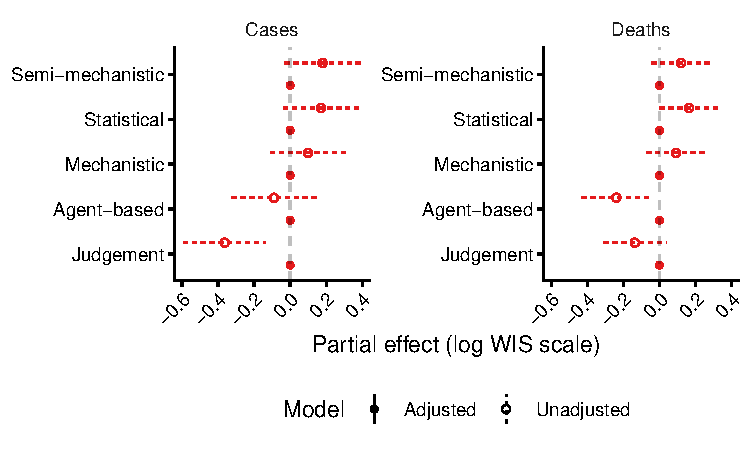
\includegraphics[keepaspectratio]{manuscript_files/figure-pdf/fig-plot-coeffs-1.pdf}}

}

\caption{\label{fig-plot-coeffs}Partial effect (95\% CI) on the weighted
interval score from model structure and geographic scope, before and
after adjustment for confounding. A lower WIS indicates better forecast
performance; effects \textless0 indicate better-than-average
performance. Adjusted effects account for forecast horizon, epidemic
trend, dominant variant phase, geographic location, and individual model
variation. Filled symbols: adjusted; open symbols: unadjusted. Partial
effects and 95\% confidence intervals estimated from a generalised
additive mixed model. WIS = weighted interval score.}

\end{figure}%

\textbf{Other drivers of forecast performance}

Among our selection of covariates, we found performance was more driven
by the target epidemiological features than by forecaster model features
(with full reporting in Supplement). Holding all other features
constant, the most predictable forecast targets appeared during periods
of stability in the epidemic curve, with better predictive performance
relative to periods of increasing or decreasing trends (cases: -0.74
(-1.47-(0)); deaths: -0.37 (-0.74-0.01)). More difficult forecasting
periods were during increasing trends in the incidence of cases (0.47
(-0.26-1.2) performance compared to stable or increasing periods).
However incident deaths were more difficult to forecast during periods
of decline (0.28 (-0.09-0.66)).

Predictability also varied between phases of variant dominance. This
influence was stronger for forecasts of case incidence than deaths,
while direction of effects was similar. We estimated better predicitive
performance during the earlier phases dominated by the Alpha and Delta
variants (Alpha cases: -0.42 (-0.64-(-0.19)), deaths: -0.1 (-0.22-0.01);
Delta cases: -0.14 (-0.36-0.09), deaths: -0.23 (-0.35-(-0.12))). We
estimated worse performance after Omicron variants became dominant (with
worse performance in the first Omicron BA.1 variant for cases: 0.33
(0.11-0.56); deaths: 0.07 (-0.04-0.19)).

We identified residual confounding, with substantial unexplained
variation between individual model performance.
Figure~\ref{fig-plot-models} shows the adjusted partial effect for each
individual model. This can be interpreted as variation in model-specific
performance after accounting for all other factors considered here. This
indicated that the variables we selected to account for variation
between forecasters (i.e.~model structure; one or multiple geographic
targets) were not sufficient to fully explain differences in
performance.

\begin{figure}

\centering{

\pandocbounded{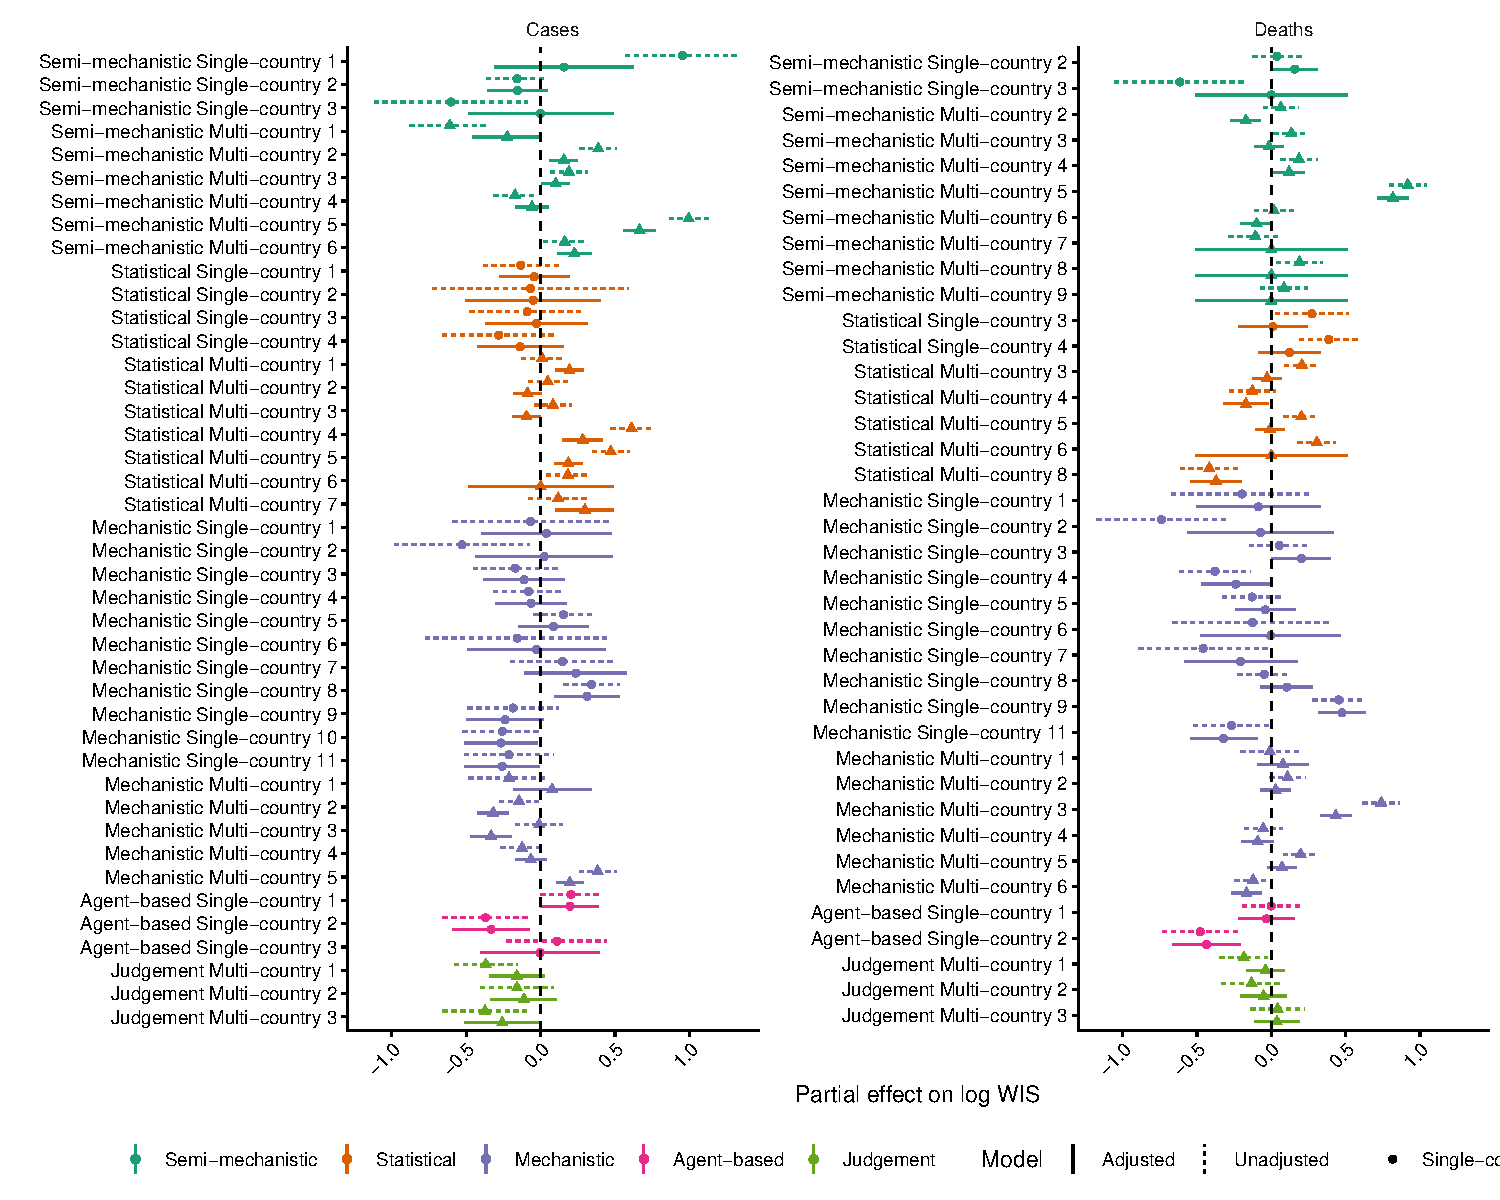
\includegraphics[keepaspectratio]{manuscript_files/figure-pdf/fig-plot-models-1.pdf}}

}

\caption{\label{fig-plot-models}Estimated partial effect size (95\% CI)
by individual model. Adjusted performance after accounting for model
structure, geographic scope, forecast horizon, epidemic trend, variant
phase, and location. Colour: model structure. Shape: geographic scope
(circle = single-country, triangle = multi-country). Remaining variation
represents unexplained heterogeneity.}

\end{figure}%

\textbf{Sensitivity analysis}

We repeated this analysis to look at performance on the natural scale
(rather than log-transformed predictions and observations), presented in
the Supplement. In developing this work, we considered several
alternative model specifications. We selected an initial set of
variables a priori, and changed this selection after updating our view
of confounding factors, for example including an effect for dominant
variant phase. We indicate these choices in the Supplement. Regardless
of a priori variable selection, we did not find any meaningful change in
partial effect sizes among alternate model specifications.

\subsubsection{Discussion}\label{discussion}

\begin{tcolorbox}[enhanced jigsaw, title=\textcolor{quarto-callout-caution-color}{\faFire}\hspace{0.5em}{TODO}, coltitle=black, colback=white, left=2mm, colbacktitle=quarto-callout-caution-color!10!white, breakable, bottomrule=.15mm, titlerule=0mm, opacityback=0, toprule=.15mm, rightrule=.15mm, arc=.35mm, toptitle=1mm, leftrule=.75mm, bottomtitle=1mm, opacitybacktitle=0.6, colframe=quarto-callout-caution-color-frame]

\begin{itemize}
\tightlist
\item[$\square$]
  note should use survival analysis
\end{itemize}

\end{tcolorbox}

In this work, we aimed to assess the influence of methodological
structure on the accuracy of infectious disease forecasts. We developed
a model-based approach to adjust for the key sources of variation in
predictive difficulty, targeting the controlled direct effect of model
structure on performance. We applied this to a multi-country multi-model
forecasting effort conducted during the COVID-19 pandemic, in order to
assess the influence of models' structure and target strategy on
forecast accuracy. Unadjusted estimates suggested differences between
model structures, but after adjustment there was little systematic
difference in average performance, with variation driven by factors
inherent to the forecast target itself.

After adjustment for confounding, we observed no systematic difference
in average performance between model structures, though substantial
variation in individual model performance remained unexplained. We
suggest that accounting for variance in epidemiological characteristics
across forecast targets is necessary for drawing meaningful comparisons
across predictive models.

However, we only partially accounted for variation among forecast
targets. For example, we noted that real-time data were frequently
updated retrospectively, with different frequencies and magnitudes
between national surveillance and reporting systems
\href{https://www.zotero.org/google-docs/?c33gx9}{(11)}.

A key limitation of this work was its limited power to detect potential
differences in performance between model structures or target
specificity. While we used a large dataset of forecasts over time, we
had a relatively small sample size of independent models and little
metadata with which to classify model structures. For example, only 3
agent-based models, where all three represented here targeted a single
country. Future work could approach this by combining data from across
multiple similar Hub projects and a more detailed assessment of the
characteristics of the model cohort.

Further, the Hub relied on an opportunistic cohort of models from
voluntary contributions. This meant our results could be biased by
unobserved characteristics that differentially affected participation,
such as the resource intensity of model development. One source of
unmeasured confounding in this setting is the latent capacity of a
forecasting team to incorporate domain expertise, which may drive both
the choice of model structure and the achievable forecast accuracy. In
addition, we did not track changes to each model's individual methods
over time, or account for this in our analysis. We did not see clear
patterns in how models changed their selection of country targets by
type of model. This helped to mitigate our concern that using a binary
classification for one or multiple targets was overly crude. A more
systematic sample of models would support a deeper investigation of
factors driving model performance.

There are likely many interactions between the effects explored here as
well as residual confounding. For example, a modeller's choice of model
structure may interact with their chosen number of targets, as in
agent-based models. Notably, different model structures may be more or
less well equipped to predict at each interval of the one to four week
forecast horizon. For example, models incorporating underlying epidemic
mechanisms may be less responsive to shorter term data artefacts but
relatively better able to demonstrate the impact of longer term
dynamics. Explicitly accounting for such interactions could be a useful
insight from future work.

Our findings are consistent with the hypothesis that variation in
forecast performance is driven more by differences among features of the
forecast target, than by differences among forecasting strategies.
Previous work has also failed to differentiate performance among model
structures, across a variety of outbreaks and epidemic dynamics
\href{https://www.zotero.org/google-docs/?4Vrj6C}{(4--6)}. Some prior
moderate evidence suggests that statistical methods gave better
performance than more mechanistic approaches
\href{https://www.zotero.org/google-docs/?pn8kMa}{(17,18,26)}. The
typical advantage of statistical models is that they capture the
autocorrelated nature of incidence time series. However, we also noted
that the more mechanistic models in our study produced a wide range of
predictive performance. This may reflect a greater range of flexibility
to incorporate forecaster experience
\href{https://www.zotero.org/google-docs/?tYe1Rg}{(18)}, and
understanding of the data generating processes that lead the forecast
target \href{https://www.zotero.org/google-docs/?2rqVL1}{(28)}: for
example, country-specific policies influencing local epidemic dynamics,
or the specific way in which the public data reflected underlying
transmission processes. While not considered here, we note the widely
replicated finding that ensemble combinations across multiple models
often produces the most reliable predictive performance
(e.g.~\href{https://www.zotero.org/google-docs/?EMHzzA}{(12,15,27)}).

Unlike past work, our conclusions are based on assessing performance
using forecasts on a log scale, rather than the natural scale of
observed data. We observed that the log scale moderated scores overall,
and in general this method appears to give less weight to penalising
inaccurate forecasts after a peak
\href{https://www.zotero.org/google-docs/?bNboAJ}{(23)}. In particular,
we saw reduced variability among the scores of semi-mechanistic models
on the log scale, compared to the natural scale.

This suggests the importance of accounting for epidemic characteristics
in assessing forecast performance, where we chose to prioritise relative
assessment of the growth rate rather than absolute counts. It remains
important to bear in mind that our conclusions towards the chosen metric
may not hold when choosing other scoring rules. We also note that we
modelled the interval score using a Gaussian error model with a
log-link. This impacted the propriety of the score as effects were
multiplicative, making estimates unsuitable for direct comparison or
ranking performance among individual models.

This points to the importance of explicitly identifying the assumptions
that underlie the method of forecast evaluation.

Alternatively, we could target the data generating process as the
outcome under evaluation. This would mean building evaluation metrics
that express a mechanistic understanding of how different processes
contribute to creating the single target timeseries. This would enable
us to identify the accuracy of different models in capturing causal
epidemic processes, rather than artefacts of the epidemic setting
\href{https://www.zotero.org/google-docs/?c33gx9}{(11)}. Different
assumptions within the evaluation metric may be useful for different
purposes, which suggests developing a more diverse portfolio approach to
evaluation methods.

Any aggregation of forecasts over time will contain within it the
autocorrelation of the timeseries. As infectious disease timeseries are
inherently highly autocorrelated, such aggregation will by default
favour statistical model structures based on estimating this
autocorrelation component.

With increasing forecasting datasets subject to evaluation, random error
decreases but bias remains. The analysis presented here is exploratory,
aimed at describing variation in forecast performance across model
structures once the most consequential sources of confounding are
accounted for. However, subsequent analysis could target the causal
estimand: pre-specifying a directed acyclic graph to derive a minimal
sufficient adjustment set of covariates, and reporting a quantitative
bias analysis (such as an E-value) for unmeasured confounding.

Accounting for confounding in this way is analogous to constraining
evaluation above a lower bound of common forecast error. This can also
be achieved by using evaluation relative to the performance of a
baseline forecaster. However, it is unclear which among multiple
possible baselines are appropriate for infectious disease forecasting
{[}@stapper, kaitlyn{]}. The selection of baseline model still faces the
question of whether to capture features that represent the data
generating process of the forecast target. In this work, we make this
process of model selection explicit by directly including these forecast
target features in a single joint estimation of performance score.

Comparisons like the one we have conducted here support a more informed
view of the role of modelling in pandemic preparedness and response.
Ultimately, improving surveillance data quality or target understanding
may yield more performance gains than advancing specific modelling
techniques.

Further model comparison projects should enable this by encouraging
methodological diversity among participants, and ensuring that detailed
structured information on model metadata (such as methodology and model
revisions) is collated alongside numerical predictions. We would
particularly encourage studies that can assess the amount of local
context that modellers use in creating or adapting their forecast model,
and similarly whether performance scales with efforts to continually
revise models, incorporate domain knowledge, or evaluate model
performance in the real-time forecasting process. Future performance
evaluations should combine information from multiple collaborative
efforts and ultimately lead to a convergence of recommendations for
which models to use when making epidemiological forecasts in an epidemic
or pandemic.

By accounting for forecast target difficulty, we adjust for the lower
bound of error set by the forecast target itself, and estimate the
realistic room for improvement from improving forecasting methods. To
estimate the effect of changing model structure alone, we then further
adjusted for forecaster selectiveness among geographic targets. We then
found that no single structural approach dominates. In this study we
contributed to better understanding the drivers of predictive
performance among forecasting models, and highlighted the importance of
appropriately adjusting for the general predictive difficulty of the
forecast target.

This work is exploratory. A fuller causal treatment would pre-specify a
directed acyclic graph, examine overlap across model-structure strata,
and provide a quantitative bias analysis for unmeasured confounding.
This work was also limited by a small sample of independent models and
likely incomplete adjustment for confounding factors. We recommend that
multi-model comparisons encourage and document their methodological
diversity, and collate detailed structured metadata on model methods
alongside numerical predictions.

\subsubsection{References}\label{references}

\begin{tcolorbox}[enhanced jigsaw, title=\textcolor{quarto-callout-caution-color}{\faFire}\hspace{0.5em}{TODO}, coltitle=black, colback=white, left=2mm, colbacktitle=quarto-callout-caution-color!10!white, breakable, bottomrule=.15mm, titlerule=0mm, opacityback=0, toprule=.15mm, rightrule=.15mm, arc=.35mm, toptitle=1mm, leftrule=.75mm, bottomtitle=1mm, opacitybacktitle=0.6, colframe=quarto-callout-caution-color-frame]

\begin{itemize}
\tightlist
\item[$\square$]
  sync with google doc zotero to bib file
\end{itemize}

\end{tcolorbox}

\begin{tcolorbox}[enhanced jigsaw, title=\textcolor{quarto-callout-caution-color}{\faFire}\hspace{0.5em}{Caution}, coltitle=black, colback=white, left=2mm, colbacktitle=quarto-callout-caution-color!10!white, breakable, bottomrule=.15mm, titlerule=0mm, opacityback=0, toprule=.15mm, rightrule=.15mm, arc=.35mm, toptitle=1mm, leftrule=.75mm, bottomtitle=1mm, opacitybacktitle=0.6, colframe=quarto-callout-caution-color-frame]

\href{https://www.zotero.org/google-docs/?7SKDbN}{1. Woolhouse M. How to
make predictions about future infectious disease risks. Philos Trans R
Soc B Biol Sci. 2011 Jul 12;366(1573):2045--54.}

\href{https://www.zotero.org/google-docs/?7SKDbN}{2. Dattner I, Huppert
A. Modern statistical tools for inference and prediction of infectious
diseases using mathematical models. Stat Methods Med Res. 2018 Jul
1;27(7):1927--9.}

\href{https://www.zotero.org/google-docs/?7SKDbN}{3. Funk S, King AA.
Choices and trade-offs in inference with infectious disease models.
Epidemics. 2020 Mar 1;30:100383.}

\href{https://www.zotero.org/google-docs/?7SKDbN}{4. Carlson CJ,
Dougherty E, Boots M, Getz W, Ryan SJ. Consensus and conflict among
ecological forecasts of Zika virus outbreaks in the United States. Sci
Rep.~2018 Mar 21;8(1):4921.}

\href{https://www.zotero.org/google-docs/?7SKDbN}{5. Viboud C, Sun K,
Gaffey R, Ajelli M, Fumanelli L, Merler S, et al.~The RAPIDD ebola
forecasting challenge: Synthesis and lessons learnt. Epidemics. 2018 Mar
1;22:13--21.}

\href{https://www.zotero.org/google-docs/?7SKDbN}{6. Reich NG, Brooks
LC, Fox SJ, Kandula S, McGowan CJ, Moore E, et al.~A collaborative
multiyear, multimodel assessment of seasonal influenza forecasting in
the United States. Proc Natl Acad Sci. 2019 Feb 19;116(8):3146--54.}

\href{https://www.zotero.org/google-docs/?7SKDbN}{7. Becker AD, Grantz
KH, Hegde ST, Bérubé S, Cummings DAT, Wesolowski A. Development and
dissemination of infectious disease dynamic transmission models during
the COVID-19 pandemic: what can we learn from other pathogens and how
can we move forward? Lancet Digit Health. 2021 Jan;3(1):e41--50.}

\href{https://www.zotero.org/google-docs/?7SKDbN}{8. Clapham H, Gad M,
Gheorghe A, Hutubessy R, Megiddo I, Painter C, et al.~Assessing
fitness-for-purpose and comparing the suitability of COVID-19
multi-country models for local contexts and users {[}Internet{]}. Gates
Open Research; 2021 {[}cited 2022 Dec 12{]}. Available from:
https://gatesopenresearch.org/articles/5-79}

\href{https://www.zotero.org/google-docs/?7SKDbN}{9. Bracher J, Wolffram
D, Deuschel J, Görgen K, Ketterer JL, Ullrich A, et al.~National and
subnational short-term forecasting of COVID-19 in Germany and Poland
during early 2021. Commun Med. 2022 Oct 31;2(1):1--17.}

\href{https://www.zotero.org/google-docs/?7SKDbN}{10. Pollett S,
Johansson M, Biggerstaff M, Morton LC, Bazaco SL, Brett Major DM, et
al.~Identification and evaluation of epidemic prediction and forecasting
reporting guidelines: A systematic review and a call for action.
Epidemics. 2020 Dec 1;33:100400.}

\href{https://www.zotero.org/google-docs/?7SKDbN}{11. Holcomb KM, Mathis
S, Staples JE, Fischer M, Barker CM, Beard CB, et al.~Evaluation of an
open forecasting challenge to assess skill of West Nile virus
neuroinvasive disease prediction. Parasit Vectors. 2023 Jan
12;16(1):11.}

\href{https://www.zotero.org/google-docs/?7SKDbN}{12. Sherratt K, Gruson
H, Grah R, Johnson H, Niehus R, Prasse B, et al.~Predictive performance
of multi-model ensemble forecasts of COVID-19 across European nations.
Wesolowski A, Ferguson NM, Shaman JL, Pei S, editors. eLife. 2023 Apr
21;12:e81916.}

\href{https://www.zotero.org/google-docs/?7SKDbN}{13. Reich NG, Lessler
J, Funk S, Viboud C, Vespignani A, Tibshirani RJ, et al.~Collaborative
Hubs: Making the Most of Predictive Epidemic Modeling. Am J Public
Health. 2022 Jun;112(6):839--42.}

\href{https://www.zotero.org/google-docs/?7SKDbN}{14. Scarpino SV, Petri
G. On the predictability of infectious disease outbreaks. Nat Commun.
2019 Feb 22;10(1):898.}

\href{https://www.zotero.org/google-docs/?7SKDbN}{15. Cramer EY, Ray EL,
Lopez VK, Bracher J, Brennen A, Castro Rivadeneira AJ, et al.~Evaluation
of individual and ensemble probabilistic forecasts of COVID-19 mortality
in the United States. Proc Natl Acad Sci. 2022 Apr
12;119(15):e2113561119.}

\href{https://www.zotero.org/google-docs/?7SKDbN}{16. Lopez VK, Cramer
EY, Pagano R, Drake JM, O'Dea EB, Adee M, et al.~Challenges of COVID-19
Case Forecasting in the US, 2020--2021. PLOS Comput Biol. 2024 May
6;20(5):e1011200.}

\href{https://www.zotero.org/google-docs/?7SKDbN}{17. Del Valle SY,
McMahon BH, Asher J, Hatchett R, Lega JC, Brown HE, et al.~Summary
results of the 2014-2015 DARPA Chikungunya challenge. BMC Infect Dis.
2018 May 30;18(1):245.}

\href{https://www.zotero.org/google-docs/?7SKDbN}{18. McGowan CJ,
Biggerstaff M, Johansson M, Apfeldorf KM, Ben-Nun M, Brooks L, et
al.~Collaborative efforts to forecast seasonal influenza in the United
States, 2015--2016. Sci Rep.~2019 Jan 24;9(1):683.}

\href{https://www.zotero.org/google-docs/?7SKDbN}{19. European Covid-19
Forecast Hub {[}Internet{]}. {[}cited 2021 Sep 1{]}. Available from:
https://covid19forecasthub.eu/index.html}

\href{https://www.zotero.org/google-docs/?7SKDbN}{20. Dong E, Du H,
Gardner L. An interactive web-based dashboard to track COVID-19 in real
time. Lancet Infect Dis. 2020 May 1;20(5):533--4.}

\href{https://www.zotero.org/google-docs/?7SKDbN}{21. Bracher J, Ray EL,
Gneiting T, Reich NG. Evaluating epidemic forecasts in an interval
format. PLOS Comput Biol. 2021 Feb 12;17(2):e1008618.}

\href{https://www.zotero.org/google-docs/?7SKDbN}{22. Bosse NI, Gruson
H, Cori A, van Leeuwen E, Funk S, Abbott S. Evaluating Forecasts with
scoringutils in R {[}Internet{]}. arXiv; 2022 {[}cited 2024 May 1{]}.
Available from: http://arxiv.org/abs/2205.07090}

\href{https://www.zotero.org/google-docs/?7SKDbN}{23. Bosse NI, Abbott
S, Cori A, Leeuwen E van, Bracher J, Funk S. Scoring epidemiological
forecasts on transformed scales. PLOS Comput Biol. 2023 Aug
29;19(8):e1011393.}

\href{https://www.zotero.org/google-docs/?7SKDbN}{24. Wood SN. Fast
Stable Restricted Maximum Likelihood and Marginal Likelihood Estimation
of Semiparametric Generalized Linear Models. J R Stat Soc Ser B Stat
Methodol. 2011 Jan 1;73(1):3--36.}

\href{https://www.zotero.org/google-docs/?7SKDbN}{25. Sherratt K, Funk
S. epiforecasts/eval-by-method: v0.1.0 {[}Internet{]}. Zenodo; 2025.
Available from: https://doi.org/10.5281/zenodo.14903162}

\href{https://www.zotero.org/google-docs/?7SKDbN}{26. Johansson MA,
Apfeldorf KM, Dobson S, Devita J, Buczak AL, Baugher B, et al.~An open
challenge to advance probabilistic forecasting for dengue epidemics.
Proc Natl Acad Sci. 2019 Nov 26;116(48):24268--74.}

\href{https://www.zotero.org/google-docs/?7SKDbN}{27. Reich NG, McGowan
CJ, Yamana TK, Tushar A, Ray EL, Osthus D, et al.~Accuracy of real-time
multi-model ensemble forecasts for seasonal influenza in the U.S. PLoS
Comput Biol. 2019 Nov;15(11):e1007486.}

\href{https://www.zotero.org/google-docs/?7SKDbN}{28. Wolffram D, Abbott
S, Heiden M an der, Funk S, Günther F, Hailer D, et al.~Collaborative
nowcasting of COVID-19 hospitalization incidences in Germany. PLOS
Comput Biol. 2023 Aug 11;19(8):e1011394.}

\subsubsection{Supporting Information}\label{supporting-information}

\textbf{Supplementary Figure 1.} Eligibility criteria for models
contributing case and death forecasts to the European COVID-19 Forecast
Hub, March 2021 - March 2023

\textbf{Supplementary Table 1.} Model characteristics contributing to
the European COVID-19 Forecast Hub, by method used, number of countries
targeted, and number of forecasts contributed

\textbf{Supplementary Figure 2.} Epidemic trends (cases)

\textbf{Supplementary Figure 3.} Epidemic trends (deaths)

\textbf{Supplementary Figure 4.} Model diagnostics (cases)

\textbf{Supplementary Figure 5.} Model diagnostics (deaths)

\subsubsection{Data availability}\label{data-availability}

The codebase for this paper is publicly available at the Github
repository ``epiforecasts/eval-by-method'' and Zenodo with DOI:
10.5281/zenodo.14903162. Forecast and observed data were sourced from
the European COVID-19 Forecast Hub, available to view online. All Hub
data are now archived at the Github repository:
``european-modelling-hubs/covid19-forecast-hub-europe\_archive'' and
Zenodo with DOI: 10.5281/zenodo.13986751. Specific data used in this
work are available in the Github repository for this paper.

\end{tcolorbox}

\subsection{Supplement}\label{supplement}

\begin{tcolorbox}[enhanced jigsaw, title=\textcolor{quarto-callout-caution-color}{\faFire}\hspace{0.5em}{TODO}, coltitle=black, colback=white, left=2mm, colbacktitle=quarto-callout-caution-color!10!white, breakable, bottomrule=.15mm, titlerule=0mm, opacityback=0, toprule=.15mm, rightrule=.15mm, arc=.35mm, toptitle=1mm, leftrule=.75mm, bottomtitle=1mm, opacitybacktitle=0.6, colframe=quarto-callout-caution-color-frame]

\begin{itemize}
\tightlist
\item[$\square$]
  check supplement includes natural scale results
\item[$\square$]
  include univariate associations of all variables
\end{itemize}

\end{tcolorbox}




\end{document}
